\documentclass[11pt]{article}
\usepackage{deauthor}
\usepackage{times}
\usepackage{wrapfig}
\usepackage{graphicx}
\usepackage{xspace}
% \usepackage[it,small]{caption}
% \usepackage[export]{adjustbox}
\usepackage{cite}
\usepackage{amsmath,amssymb,amsfonts}
\usepackage{textcomp}
\usepackage{graphicx}
\usepackage{algorithm}
\usepackage{algorithmic}
\usepackage{xcolor}


% ensure times
\usepackage{txfonts}
\usepackage{url}

\usepackage{balance}  % for  \balance command ON LAST PAGE  (only there!)
\usepackage{booktabs} % For formal tables
\usepackage{enumitem}
\usepackage{multirow}
\usepackage{subcaption}
\usepackage{authblk}

% \usepackage[pdfpagelabels=false]{hyperref}

\usepackage{listings}

\usepackage{outlines}



% Break URLs properly

\title{The Road for Recovery: 
Aligning COVID-19 efforts and building a more resilient future}

\author{Meredith M. Lee, Alicia D. Johnson, Katherine A. Yelick, and Jennifer T. Chayes
\\
UC Berkeley Division of Computing, Data Science, and Society, \\
West Big Data Innovation Hub, \\
UC Berkeley Office of Emergency Management, \\
UC Berkeley Department of Electrical Engineering and Computer Sciences, \\
and Lawrence Berkeley National Laboratory}

\begin{document}

\maketitle

%\begin{abstract}
%Governments around the world have become increasingly frustrated with tech giants dictating public health policy. The software created by Apple and Google enables individuals to track their own potential exposure through collated exposure notifications. However, the same software prohibits location tracking, denying key information needed by public health officials for robust contract tracing. This information is needed to treat and isolate COVID-19 positive people, identify transmission hotspots, and protect against continued spread of infection.
%In this article, we present two simple ideas: the \textbf{lighthouse} and the \textbf{covid-commons} that address the needs of public health authorities while preserving the privacy-sensitive goals of the Apple and google exposure notification protocols. 
%\end{abstract}


\section{A Pivotal Moment}
% Based on this Google Doc: 
% https://docs.google.com/document/d/1pJMU7AzuoaGf7Kegx8K9HmPANkRP2mbsWYEfkA722Cc/edit?usp=sharing


Our society currently faces the most profound and deeply disruptive public health crisis in modern history. As communities across the world grapple with the COVID-19 pandemic, scientific advances spanning biochemistry and epidemiology to manufacturing and data engineering offer hope—and a spectrum of guidance is unfolding in an effort to respond to monumental shifts in our daily lives. The rising demand for data and the emerging efforts to responsibly collect, share, and analyze information across traditional boundaries play a vital role in our next steps.  

From facilitating dialogue and decision making, to underscoring the importance of a shared, honest assessment of where we are in our collective fight against the pandemic, data are now more important than ever. Our computational capacity and the value that we as a community can generate through data science are fundamentally crucial to our resilience. As we look to transition from crisis response to longer-term recovery, we have an unprecedented opportunity to re-imagine a new data-enabled future.

\begin{figure}
    \centering
    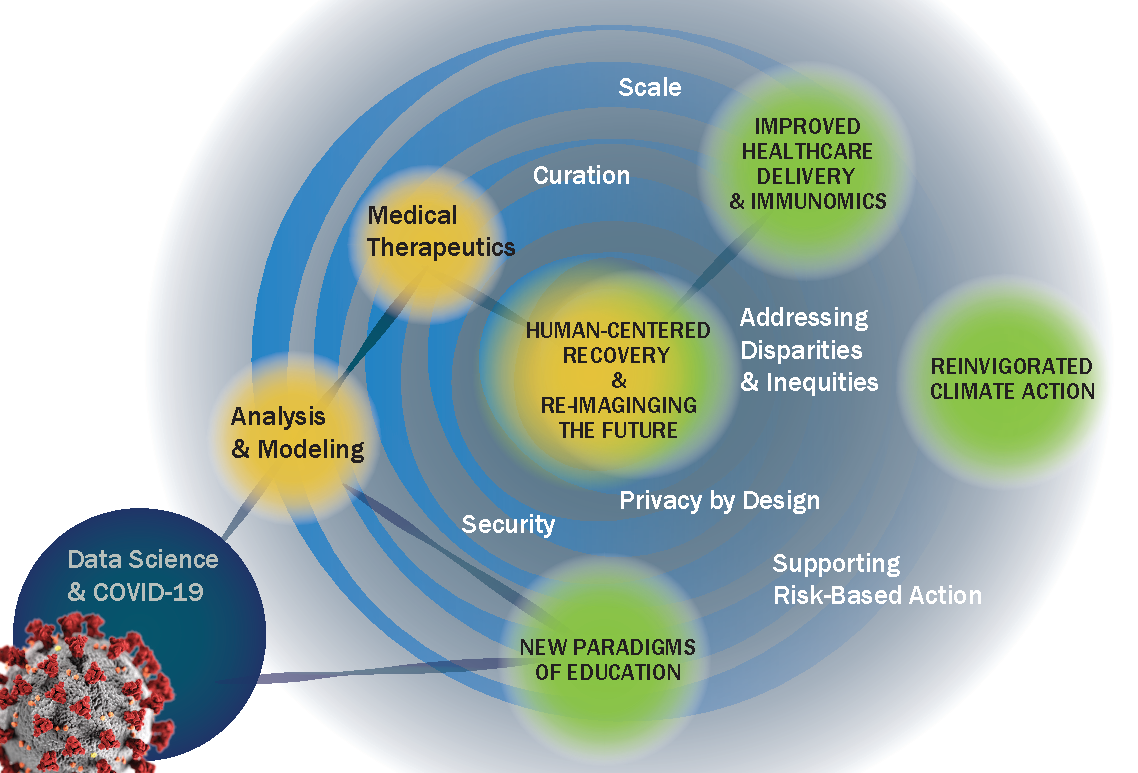
\includegraphics[width=0.75\textwidth]{figs/covid19_landscape.pdf}
    \caption{\textbf{Supporting Public Health.} The COVID-19 pandemic surfaces challenges where data science can enable new insights within a human-centered context. Current efforts, ranging from data analysis and predictive modeling to risk communication, set the stage for recovery and a new future, reinvigorated with critical questions and opportunities.}
  %  \label{fig:placesExamples}
\end{figure}



\section{Emerging Research: The Challenge of the Unknown}

Our landscape has shifted, and our paths forward will require unparalleled levels of creativity, persistence, and humility as we strengthen connections across sectors and disciplines, translating ideas into action. 
Although the data are rarely complete and extracting useful signals from the noise can be elusive, a number of COVID-19 data-enabled research efforts are emerging, including:

\subsection*{Analysis and Modeling}
Considerable emphasis on data analysis and modeling has spurred discussion that bridges statistical methods, machine learning, and artificial intelligence with policy development and risk communication~\cite{Lewnardm1923, best_boice_2020, institute, covidactnow}. 
For example, N. Alteri et al. have developed several predictors after curating available data, collaborating with nonprofit organizations and healthcare providers to address medical supply needs for individual hospitals~\cite{altieri2020curating}. 
U. Seljak et al. have employed robust statistical methods to identify systematic errors and correct mortality rates that are integral to further analysis~\cite{Modi2020.04.15.20067074}, while S. Yadlowsky et al. have modeled the infection prevalence of the virus~\cite{Yadlowsky2020.03.24.20043067}, with J. Steinhardt and A. Ilyas noting shortcomings of existing tracking measures~\cite{steinhardt}. 

Such efforts can help communities visualize the nature of fluid events and iteratively explore reasonable response strategies when faced with unprecedented scenarios. Notably, as communities across the globe adjust their behavior against a backdrop of changing policies, guidance, and tactics, we have an opportunity to improve our assessments about the spread of the virus and to understand how our actions and other factors relate to key outcomes. Intentional and thoughtful data collection and analysis during recovery, focused on public health risks and implications—and acknowledging the critical lag between knowledge and informed action—will be of paramount importance.

\subsection*{Exploration to Aid Medical Therapeutics}
As researchers and medical professionals from a variety of disciplines seek to accelerate actionable knowledge, collaborative frameworks and data exploration efforts are forming. National laboratories and science centers are searching databases for drug candidates that could be re-purposed for COVID-19 or used to inform clinical practice, sharing and updating progress more rapidly than traditional publication timeframes~\cite{Smith2020, Chen2020.04.17.047548}. Consortia aiming to speed dialogue and visualization of SARS-CoV-2 genomes through open online reports~\cite{nextstrain}, as well as clinical study groups and collaborators working together in new ways, have the potential to shape and improve diagnostics, vaccine development, and outcomes~\cite{schneider2019rethinking, kaggle}. 

\section{Shared Human-Centered Context: The Need To Explore Difficult Questions, Together}

As our collective response to the pandemic evolves, openly updating and sharing code, data, and insights as they develop is particularly critical for scientific reproducibility and effective coordination. Yet, a tension exists when evaluating the quality of information and choosing how to provide data, analysis, or tools to others. Noting the importance of clear, accurate, updated, and actionable information, the State of California coronavirus response team published a Digital Crisis Standard~\cite{crisisstandard} with principles and framing questions that highlight accessibility, interoperability, and a focus on user needs and accountability. 

Indeed, in the realm of disaster response and recovery, essential questions and unexplored frontiers arise in a fundamentally human-centered context. Issues stemming from ethics concerns and socioeconomic implications \emph{must} be addressed early and often. Existing frameworks, theories, and practices that cut across disciplines are being put to the test and reconsidered as we face COVID-19, including:

\subsection*{Incorporating Privacy by Design}
Adopted by the International Assembly of Privacy Commissioners and Data Protection Authorities nearly a decade ago, the foundational principles of the Privacy by Design framework~\cite{cavoukian2013privacy} build upon views and practices emphasizing proactive, “by default”, and embedded mechanisms that respect user privacy. With a backdrop of the General Data Protection Regulation and increasing prevalence of data privacy acts, laws, and norms~\cite{GDPR, mares2019iot}, emerging work towards privacy-sensitive proximity contact tracing looks to enable data exchange without compromising civil liberties, to query encrypted data, and to comply with unfolding guidelines for privacy safeguards~\cite{FPF}.

Sharing information that could be relevant for individual or community health outcomes surfaces a number of deeper questions, where personal sentiment and expectations can vary widely. \emph{What information should remain private, under what circumstances? What might I share in hopes of helping others? Will my privacy preferences change? Am I empowered to make choices about my privacy and data?} The tensions surrounding privacy and nuances around data sharing, while not new by any means~\cite{10.1007/3-540-45427-6_23, 10.1145/642611.642635}, are integral to our COVID-19 response and recovery.   

\subsection*{Addressing Disparities and Inequities}
With increased capacity to view data about disease incidence and mortality across demographic information, analysis showing disproportionate COVID-19 impacts on black communities, Latinx communities, and additional historically marginalized groups has surfaced~\cite{covidrace}. Z. Obermeyer et al. have noted how existing measures can obscure rather than demonstrate inequality~\cite{Obermeyer447}. For example, communities with less access to testing for SARS-CoV-2 will have fewer diagnosed cases, making the epidemic look less severe. This can lead to disparities in attention and funding, and distort algorithms meant to help. 

Networks of government cohorts have featured data-driven equity visualization tools and are increasingly convening public discussions focused on inclusion, a sense of belonging, and equity~\cite{GARE}. In order to support meaningful change, we will need to find ways to support empathy and shared understanding, directing energy towards measurable improvements. Partnerships to enable data compilation, analysis, and deeper research are essential, but we will need to leverage our ingenuity holistically and hold ourselves accountable to the bigger picture. \emph{What levers do we have to address systemic issues? Who is missing from the conversation? How might we support public awareness, engagement, and education, creatively?} 

Globally, with 265 million people projected to suffer from acute hunger by the end of this year, data-driven analysis is creating new options to help mitigate the most devastating impacts of COVID-19 in low- and middle-income countries.  For example, applications of machine learning to satellite imagery and mobile phone data are helping identify those individuals most in need of immediate humanitarian aid, and complement conventional methods that are limited by a lack of reliable and up-to-date data~\cite{blumenstock2020machine, blumenstock2016fighting}. 

\subsection*{Mechanisms for Supporting Risk-Based Action}
Design through the lens of risk underscores the need to better quantify and qualify threats, vulnerabilities, and consequences. Throughout the pandemic, the corpus of available information and the assessment of risk are continuously changing as more is discovered about the virus and how it interacts with our communities. In a world where the opportunity for technology-driven situational awareness during a crisis is strikingly juxtaposed with an “infodemic” of extensive misinformation and dis-information~\cite{zade, UN, Hany}, we are starving for transparent, appropriately vetted, and curated information in context.  

In the clinical setting, aggregating data to capture patient risk indices could help communities more methodically assess and navigate difficult situations with new information, but effectively focusing attention and limited resources towards optimized patient outcomes remains an ongoing, and often overwhelming, challenge ~\cite{zhou2020clinical, onder2020case}. In all too many cases, the pandemic is exacerbating existing vulnerabilities. Any “solutions” or approaches need to consider the nature of risks and how risk evolves over time.  


\section{Compound Disasters and Interdependencies}

Moreover, as the pandemic extends, the likelihood that additional communities will be impacted by both COVID-19 and compounded disasters—such as wildfires, hurricanes, earthquakes or tornadoes—is increasingly high. The U. S. Federal Emergency Management Agency (FEMA) has published guidance to prepare State, Local, Tribal, and Territorial (SLTT) responders to adapt their response and recovery procedures to this new combination of threats. The COVID-19 Pandemic Operational Guidance for the 2020 Hurricane Season (May 2020) notes the need for response and recovery adaptation that includes virtual damage assessments and significant reliance on the “whole of community” (including the private and non-profit sectors) to maximize their abilities to respond to simultaneously occurring disasters~\cite{FEMAPOG}. 

While in any given year, national-scale agencies managing emergencies routinely respond to multiple disasters simultaneously, SLTT responders often respond to one devastation at a time. Local economies strained by COVID-19 create an inability for communities to truly prepare and protect themselves from all impending hazards. Communities unable to protect themselves may suffer additional strain and damage that makes recovery from the compounded disaster even further from reach.

In an effort to proactively acknowledge limitations, the U.S. National Interagency Fire Coordination Center notes in its May 2020 plans, “In the event of a high disease spread scenario with a high rate of infection, the associated loss of individuals from service will severely tax the ability to maintain an adequate wildfire response, even during a moderately active fire season”. The need for adaptation and re-orienting plans in light of COVID-19 extends to all hazards, as the methodologies and tools SLTT decision makers and responders currently use do not conform to physical distancing guidance and may amplify concerns about responder long-term health.  

Moreover, some communities’ plans and capabilities are not robust to damaged infrastructure or limited internet capacity, rendering strategies for multiple in-depth virtual interactions ineffective at best. Our reflections and how we navigate these challenges promise to impact our communities long after the virus has run its course. 

While the movement to “flatten the curve” offered fairly uniform and straightforward guidance, to shelter in place and physically distance, the road for recovery and the notion of what a “new normal” looks like is riddled with additional interdependencies and tensions. These multifaceted challenges are increasingly being addressed through diverse coalitions, for example, with State-level economic development agencies working alongside university researchers, healthcare institutions, and volunteers to develop and share data, rapidly register products, and mitigate risks as guidance and authorizations evolve~\cite{doi:10.1056/NEJMc2009432,western}.




\section{Re-imagining Resilience}
With such a complex backdrop, it is more critical than ever to consider the roles for computing in social change ~\cite{abebe2020roles} along with ethical implications~\cite{stoyan, gotterbarn2017acm, bloomberg, EthicalOS, Guidebook} to enable response—responsibly.  Data scientists and data enthusiasts globally have immense potential to light the path towards:

\subsection*{Improved Healthcare Delivery and Accelerated Growth of Immunomics}
The pandemic has surfaced severe inadequacies in healthcare systems worldwide. New approaches to healthcare delivery must incorporate current lessons learned, and context, to address the fundamental needs of local communities and strive for measurable reductions in racial and economic biases. \emph{How might we meet individuals and communities where they are, culturally and metaphorically? How can we imagine and achieve equitable health services across numerous barriers that exist today?} These framing questions should keep us grounded as exciting advances in computational immunomics promise to not only mitigate the effects of new viruses, but also provide novel treatments for autoimmune diseases, cancer, and other conditions. 
 
\subsection*{Reinvigorated Climate Action}
The dramatically altered global patterns of transportation and energy use during the pandemic will allow us to imagine new methods of interacting with each other and our environment. With many international and local borders closed for non-essential activity, and individual confinement extending, we have an opportunity to revisit the impacts of both policy and behavior changes on greenhouse gas emissions, our natural resources, and our clean energy economy~\cite{le2020temporary}. Worldwide, individuals and organizations have a chance to reflect on our choices and climate commitments. Moreover, the pandemic continues to expose the lack of safe, accessible water in underserved rural as well as urban areas, raising opportunities to support equitable infrastructure investment and environmental justice. 
 
\subsection*{New Paradigms of Online Education}
Our concept of how we learn and the future of work may be forever changed. Online learning, once viewed as a less-prestigious option relevant only to a subset of students, is now at least temporarily the norm across the globe, for students from preschool through doctoral programs and in continuing and executive education. Ensuring that \emph{all} students have access to appropriate hardware, software, internet connectivity, and resources to support distance learning is critical~\cite{UCBinterview, Jenna, Pardos}. 
As remote teaching and learning extends, further research on the impacts of adopting new technologies—spanning issues from student privacy, safety, and mental health to the metacognitive aspects of learning, including motivation, resiliency, persistence, and scaffolding, will be needed. We must also be mindful of demands on instructors; training in new methods and logistical support for teachers should become a social priority. Experts, institutions, and authorities who are able to do so should share resources for effective and responsible distance learning widely, following open source models~\cite{unesco}.



\section{Conclusion}While our community will surely grapple with unanticipated complexities over the next weeks, months, and years, we have a call-to-action in this moment and a hope for building a more resilient future. The future needs us to learn from the past and present—to deploy an inherently human-centered approach that connects research with the realities of crisis management, long-term recovery, and the vulnerabilities of being human. The future needs us to ask \emph{Can we?} and \emph{Should we?} as we learn how to harness the full potential of our collective resources. 
\subsubsection*{Acknowledgements} The authors would like to acknowledge the dedicated individuals contributing to UC Berkeley’s COVID-19 response, especially Jennifer Doudna, Michael Lu, Maya Petersen, Art Reingold, Anna Harte, Guy Nicolette, Fyodor Urnov, David Culler, and Joseph Gonzalez.  In addition, M. Lee thanks collaborators from the Obama Administration White House Innovation for Disaster Response and Recovery Initiative and the National Science and Technology Council Subcommittee on Disaster Reduction. A. Johnson would like to thank the innumerable collaborations with local jurisdictions and communities that diligently remind her of the “why” behind the work of emergency management. Finally, the authors thank the National Science Foundation and network of regional data innovation hubs for efforts to spark and scale translational data science activities addressing societal needs. 


% \bibliographystyle{IEEEtran}
% \bibliography{references}


% Generated by IEEEtran.bst, version: 1.14 (2015/08/26)
\begin{thebibliography}{10}
\providecommand{\url}[1]{#1}
\csname url@samestyle\endcsname
\providecommand{\newblock}{\relax}
\providecommand{\bibinfo}[2]{#2}
\providecommand{\BIBentrySTDinterwordspacing}{\spaceskip=0pt\relax}
\providecommand{\BIBentryALTinterwordstretchfactor}{4}
\providecommand{\BIBentryALTinterwordspacing}{\spaceskip=\fontdimen2\font plus
\BIBentryALTinterwordstretchfactor\fontdimen3\font minus
  \fontdimen4\font\relax}
\providecommand{\BIBforeignlanguage}[2]{{%
\expandafter\ifx\csname l@#1\endcsname\relax
\typeout{** WARNING: IEEEtran.bst: No hyphenation pattern has been}%
\typeout{** loaded for the language `#1'. Using the pattern for}%
\typeout{** the default language instead.}%
\else
\language=\csname l@#1\endcsname
\fi
#2}}
\providecommand{\BIBdecl}{\relax}
\BIBdecl

\bibitem{Lewnardm1923}
J.~A. Lewnard~et al., ``{Incidence, clinical outcomes, and transmission
  dynamics of severe coronavirus disease 2019 in California and Washington:
  prospective cohort study},'' \emph{BMJ}, vol. 369, 2020.

\bibitem{best_boice_2020}
\BIBentryALTinterwordspacing
R.~Best and J.~Boice, ``{Where the latest COVID-19 models think we're headed -
  and why they disagree},'' May 2020. [Online]. Available:
  \url{https://projects.fivethirtyeight.com/covid-forecasts/}
\BIBentrySTDinterwordspacing

\bibitem{institute}
\BIBentryALTinterwordspacing
``{Institute for Health Metrics and Evaluation}.'' [Online]. Available:
  \url{http://www.healthdata.org/}
\BIBentrySTDinterwordspacing

\bibitem{covidactnow}
\BIBentryALTinterwordspacing
``{CovidActNow.org}.'' [Online]. Available: \url{https://www.covidactnow.org/}
\BIBentrySTDinterwordspacing

\bibitem{altieri2020curating}
\BIBentryALTinterwordspacing
N.~Altieri~et al., ``{Curating a COVID-19 data repository and forecasting
  county-level death counts in the United States},'' 2020. [Online]. Available:
  \url{https://arxiv.org/abs/2005.07882}
\BIBentrySTDinterwordspacing

\bibitem{Modi2020.04.15.20067074}
\BIBentryALTinterwordspacing
C.~Modi, V.~Boehm, S.~Ferraro, G.~Stein, and U.~Seljak, ``{How deadly is
  COVID-19? A rigorous analysis of excess mortality and age-dependent fatality
  rates in Italy},'' \emph{medRxiv}, 2020. [Online]. Available:
  \url{https://www.medrxiv.org/content/early/2020/05/14/2020.04.15.20067074}
\BIBentrySTDinterwordspacing

\bibitem{Yadlowsky2020.03.24.20043067}
\BIBentryALTinterwordspacing
S.~Yadlowsky, N.~Shah, and J.~Steinhardt, ``{Estimation of SARS-CoV-2 infection
  prevalence in Santa Clara County},'' \emph{medRxiv}, 2020. [Online].
  Available:
  \url{https://www.medrxiv.org/content/early/2020/03/27/2020.03.24.20043067}
\BIBentrySTDinterwordspacing

\bibitem{steinhardt}
\BIBentryALTinterwordspacing
J.~Steinhardt and A.~Ilyas, ``{Prevalence tracking mechanisms for
  SARS-CoV-2},'' (Accessed 29 May 2020). [Online]. Available:
  \url{http://web.archive.org/web/20200529022542/https://www.stat.berkeley.edu/~jsteinhardt/publications/CovidPrevalenceTracking.pdf}
\BIBentrySTDinterwordspacing

\bibitem{Smith2020}
\BIBentryALTinterwordspacing
M.~Smith and J.~C. Smith, ``{Repurposing therapeutics for COVID-19:
  Supercomputer-based docking to the SARS-CoV-2 viral spike protein and viral
  spike protein-human ACE2 interface},'' 3 2020. [Online]. Available:
  \url{https://chemrxiv.org/articles/Repurposing_Therapeutics_for_the_Wuhan_Coronavirus_nCov-2019_Supercomputer-Based_Docking_to_the_Viral_S_Protein_and_Human_ACE2_Interface/11871402}
\BIBentrySTDinterwordspacing

\bibitem{Chen2020.04.17.047548}
\BIBentryALTinterwordspacing
S.~H. Chen, M.~T. Young, J.~Gounley, C.~Stanley, and D.~Bhowmik, ``{Distinct
  structural flexibility within SARS-CoV-2 spike protein reveals potential
  therapeutic targets},'' \emph{bioRxiv}, 2020. [Online]. Available:
  \url{https://www.biorxiv.org/content/early/2020/04/18/2020.04.17.047548}
\BIBentrySTDinterwordspacing

\bibitem{nextstrain}
\BIBentryALTinterwordspacing
``{Nextstrain.org},'' (Accessed 29 May 2020). [Online]. Available:
  \url{http://web.archive.org/web/20200529023700/https://nextstrain.org/ncov-sit-reps/}
\BIBentrySTDinterwordspacing

\bibitem{schneider2019rethinking}
P.~Schneider~et al., ``Rethinking drug design in the artificial intelligence
  era,'' \emph{Nature Reviews Drug Discovery}, pp. 1--12, 2019.

\bibitem{kaggle}
\BIBentryALTinterwordspacing
``{kaggle CORD-19 Research Challenge},'' (Accessed 29 May 2020). [Online].
  Available:
  \url{http://web.archive.org/web/20200529015651/https://www.kaggle.com/allen-institute-for-ai/CORD-19-research-challenge}
\BIBentrySTDinterwordspacing

\bibitem{crisisstandard}
\BIBentryALTinterwordspacing
``{Digital Crisis Standard - covid19.ca.gov},'' (Accessed 15 May 2020).
  [Online]. Available:
  \url{http://web.archive.org/web/20200515011426/https://github.com/cagov/covid19/wiki/Crisis-standard}
\BIBentrySTDinterwordspacing

\bibitem{cavoukian2013privacy}
A.~Cavoukian, ``Privacy by design: leadership, methods, and results,'' in
  \emph{European Data Protection: Coming of Age}.\hskip 1em plus 0.5em minus
  0.4em\relax Springer, 2013, pp. 175--202.

\bibitem{GDPR}
\BIBentryALTinterwordspacing
``{General Data Protection Regulation}.'' [Online]. Available:
  \url{https://ec.europa.eu/commission/priorities/
  justice-and-fundamental-rights/data-protection/2018-reform-eu-data-protection-rules_en}
\BIBentrySTDinterwordspacing

\bibitem{mares2019iot}
C.~D. Mares, ``{IoT: Privacy, security, and your civil rights},'' in
  \emph{Women Securing the Future with TIPPSS for IoT}.\hskip 1em plus 0.5em
  minus 0.4em\relax Springer, 2019, pp. 15--36.

\bibitem{FPF}
\BIBentryALTinterwordspacing
G.~Zanfir-Fortuna, ``{European Union’s data-based policy against the
  pandemic, explained},'' (Accessed 29 May 2020). [Online]. Available:
  \url{http://web.archive.org/web/20200529042315/https://fpf.org/2020/04/30/european-unions-data-based-policy-against-the-pandemic-explained/}
\BIBentrySTDinterwordspacing

\bibitem{10.1007/3-540-45427-6_23}
M.~Langheinrich, ``Privacy by design - principles of privacy-aware ubiquitous
  systems,'' in \emph{Ubiquitous Computing}, G.~D. Abowd, B.~Brumitt, and
  S.~Shafer, Eds.\hskip 1em plus 0.5em minus 0.4em\relax Berlin: Springer,
  2001, pp. 273--291.

\bibitem{10.1145/642611.642635}
L.~Palen and P.~Dourish, ``Unpacking “privacy” for a networked world,'' in
  \emph{Proceedings of the SIGCHI Conference on Human Factors in Computing
  Systems}, 2003, p. 129–136.

\bibitem{covidrace}
\BIBentryALTinterwordspacing
``{The COVID Racial Data Tracker}.'' [Online]. Available:
  \url{https://covidtracking.com/race}
\BIBentrySTDinterwordspacing

\bibitem{Obermeyer447}
Z.~Obermeyer, B.~Powers, C.~Vogeli, and S.~Mullainathan, ``Dissecting racial
  bias in an algorithm used to manage the health of populations,''
  \emph{Science}, vol. 366, no. 6464, pp. 447--453, 2019.

\bibitem{GARE}
\BIBentryALTinterwordspacing
``{Government Alliance on Race and Equity}.'' [Online]. Available:
  \url{https://www.racialequityalliance.org/}
\BIBentrySTDinterwordspacing

\bibitem{blumenstock2020machine}
J.~Blumenstock, ``{Machine learning can help get COVID-19 aid to those who need
  it most},'' \emph{Nature}, 2020.

\bibitem{blumenstock2016fighting}
J.~E. Blumenstock, ``Fighting poverty with data,'' \emph{Science}, vol. 353,
  no. 6301, pp. 753--754, 2016.

\bibitem{zade}
\BIBentryALTinterwordspacing
H.~Zade, K.~Shah, V.~Rangarajan, P.~Kshirsagar, M.~Imran, and K.~Starbird,
  ``From situational awareness to actionability: Towards improving the utility
  of social media data for crisis response,'' \emph{Proc. ACM Hum.-Comput.
  Interact.}, vol.~2, no. CSCW, Nov. 2018. [Online]. Available:
  \url{https://doi.org/10.1145/3274464}
\BIBentrySTDinterwordspacing

\bibitem{UN}
\BIBentryALTinterwordspacing
``{UN tackles ‘infodemic’ of misinformation and cybercrime in COVID-19
  crisis}.'' [Online]. Available:
  \url{http://web.archive.org/web/20200529050148/https://www.un.org/}
\BIBentrySTDinterwordspacing

\bibitem{Hany}
S.~J. Nightingale, M.~Faddoul, and H.~Farid, ``{Quantifying the reach and
  belief in COVID-19 misinformation},'' in press.

\bibitem{zhou2020clinical}
F.~Zhou~et al., ``{Clinical course and risk factors for mortality of adult
  inpatients with COVID-19 in Wuhan, China: a retrospective cohort study},''
  \emph{The Lancet}, 2020.

\bibitem{onder2020case}
G.~Onder, G.~Rezza, and S.~Brusaferro, ``{Case-fatality rate and
  characteristics of patients dying in relation to COVID-19 in Italy},''
  \emph{JAMA}, vol. 323, no.~18, pp. 1775--1776, 2020.

\bibitem{FEMAPOG}
\BIBentryALTinterwordspacing
{U.S. Department of Homeland Security, Federal Emergency Management Agency},
  ``{COVID-19 Pandemic Operational Guidance for the 2020 Hurricane Season}.''
  [Online]. Available:
  \url{https://www.fema.gov/media-library-data/1589997234798-adb5ce5cb98a7a89e3e1800becf0eb65/2020_Hurricane_Pandemic_Plan.pdf}
\BIBentrySTDinterwordspacing

\bibitem{doi:10.1056/NEJMc2009432}
\BIBentryALTinterwordspacing
M.~L. Zeidel, C.~Kirk, and B.~Linville-Engler, ``Opening up new supply
  chains,'' \emph{New England Journal of Medicine}, vol. 382, no.~21, p. e73,
  2020. [Online]. Available: \url{https://doi.org/10.1056/NEJMc2009432}
\BIBentrySTDinterwordspacing

\bibitem{western}
\BIBentryALTinterwordspacing
``{California, Oregon, and Washington announce western states pact}.''
  [Online]. Available:
  \url{https://www.gov.ca.gov/2020/04/13/california-oregon-washington-announce-western-states-pact/}
\BIBentrySTDinterwordspacing

\bibitem{abebe2020roles}
R.~Abebe, S.~Barocas, J.~Kleinberg, K.~Levy, M.~Raghavan, and D.~G. Robinson,
  ``Roles for computing in social change,'' in \emph{Proceedings of the 2020
  Conference on Fairness, Accountability, and Transparency}, 2020, pp.
  252--260.

\bibitem{stoyan}
J.~Stoyanovich, B.~Howe, S.~Abiteboul, G.~Miklau, A.~Sahuguet, and G.~Weikum,
  ``Fides: Towards a platform for responsible data science,'' in
  \emph{Proceedings of the 29th International Conference on Scientific and
  Statistical Database Management}, 2017.

\bibitem{gotterbarn2017acm}
D.~Gotterbarn, A.~Bruckman, C.~Flick, K.~Miller, and M.~J. Wolf, ``{ACM code of
  ethics: a guide for positive action},'' \emph{Communications of the ACM},
  vol.~61, no.~1, pp. 121--128, 2017.

\bibitem{bloomberg}
L.~Erickson, N.~Evans~Harris, and M.~M. Lee, ``It's time for data ethics
  conversations at your dinner table,'' \emph{Tech at Bloomberg}, 2018.

\bibitem{EthicalOS}
\BIBentryALTinterwordspacing
{Omidyar Network and the Institute for the Future}, ``The ethical operating
  system.'' [Online]. Available: \url{https://ethicalos.org/}
\BIBentrySTDinterwordspacing

\bibitem{Guidebook}
\BIBentryALTinterwordspacing
N.~Evans~Harris, ``Sharing data for social impact: Guidebook to establishing
  responsible governance practices.'' [Online]. Available:
  \url{https://beeckcenter.georgetown.edu/wp-content/uploads/2020/01/Data-Sharing-Report.pdf}
\BIBentrySTDinterwordspacing

\bibitem{le2020temporary}
C.~Le~Qu{\'e}r{\'e}~et al., ``{Temporary reduction in daily global CO2
  emissions during the COVID-19 forced confinement},'' \emph{Nature Climate
  Change}, pp. 1--7, 2020.

\bibitem{UCBinterview}
\BIBentryALTinterwordspacing
E.~Lempinen, ``The pandemic could open a door to new technology — and
  dramatic innovation — in education,'' 2020. [Online]. Available:
  \url{http://web.archive.org/web/20200530235421/https://news.berkeley.edu/2020/05/27/the-pandemic-could-open-a-door-to-new-technology-and-dramatic-innovation-in-education/}
\BIBentrySTDinterwordspacing

\bibitem{Jenna}
\BIBentryALTinterwordspacing
J.~Burrell, ``{The value of the internet to rural populations: a case study
  from Mendocino County, CA},'' 2016. [Online]. Available:
  \url{https://web.archive.org/web/20200530234610/http://www.mendocinobroadband.org/wp-content/uploads/Jenna-Rural-Internet-Report.pdf}
\BIBentrySTDinterwordspacing

\bibitem{Pardos}
\BIBentryALTinterwordspacing
Z.~Pardos, ``{What to look for in online learning apps for K-12},'' 2020.
  [Online]. Available:
  \url{http://web.archive.org/web/20200530235325/https://gse.berkeley.edu/news/what-look-online-learning-apps-k-12}
\BIBentrySTDinterwordspacing

\bibitem{unesco}
\BIBentryALTinterwordspacing
{United Nations Educational Scientific and Cultural Organization}, ``Supporting
  learning and knowledge sharing through open educational resources,'' 2020.
  [Online]. Available:
  \url{http://web.archive.org/web/20200511005825/https://en.unesco.org/sites/default/files/covid19_joint_oer_call_en.pdf}
\BIBentrySTDinterwordspacing

\end{thebibliography}



\end{document}
